%!TEX root = these.tex

\chapter[La Réalité Virtuelle et la Biologie Structurale : usages, enjeux et persectives]{La Réalité Virtuelle et la Biologie Structurale : usages, enjeux et persectives}
\label{Sec:visuAna}
\minitoc
\cleardoublepage

%% Commentaire : la commande \texorpdfstring permet de déclarer un titre de
%% chapitre (ou section, sous-section) alternatif en texte seul, si besoin, qui
%% est utilisé par hyperref pour fabriquer un menu dans les fichiers compilés

%\chapter{\texorpdfstring{Contrôle gestuel de l'articulation}{Contrôle gestuel de l'articulation}}
%% Commentaire : la commande \texorpdfstring permet de déclarer un titre de
%% chapitre (ou section, sous-section) alternatif en texte seul, si besoin, qui
%% est utilisé par hyperref pour fabriquer un menu dans les fichiers compilés

%Exemple de notation qui sera reprise dans l'index : soit $\Q$\index{Q@$\Q$} le corps des nombres rationnels.


%Comme cela est le cas pour les outils de modélisation moléculaire, il est important d'amener les outils de visualisation à s'intégrer aux efforts de développement reflétés dans les technologies de pointe développées ces 10 dernières années. La démocratisation de ces dernières va ouvrir de nouvelles habitudes d'utilisation qui doivent être anticipées, que ce soit au sein des processus d'enseignement, de recherche ou bien de développement. Parmi les nouvelles technologies possédant un impact potentiel fort sur la biologie structurale, nous avons vu que la \textbf{Réalité Virtuelle} (RV) est un candidat idéal pour répondre à certaines des problématiques évoquées dans le chapitre précédent (voir section \ref{limits_persp_bio_struct}). Les investissements dans ce domaine sont conséquents et le fleurissement des projets de casques de RV par les plus grandes compagnies internationales de haute technologie (Facebook/Occulus, Samsung Gear VR, HTC Vive, Morpheus de Sony, etc.) au cours de ces derniers mois est la preuve d'un engouement général pour ces nouvelles technologies.


Les contributions de la Réalité Virtuelle (RV) pour résoudre des problématiques industrielles et scientifiques sont depuis quelques années de plus en plus nombreuses. Cet essor peut être expliqué par deux facteurs principaux : (1) la démocratisation des dispositifs de visualisation et d'interaction issus de la réalité virtuelle et augmentée et (2) l'apport de la 3d pour observer et manipuler des objets massives complexes intrinsèquement tridimensionnelles. Le besoin conjoint de mieux percevoir et de manipuler les objets tridimensionnels que constituent les structures moléculaires de manière plus efficace, a abouti à une appropriation assez rapide de techniques de Réalité Virtuelle comme la stéréoscopie par la communauté de biologie molécualaire. Dans ce chapitre, aorès quelques définitions nous décrirons plus en détail les apports de la Réalité Virtuelle pour la biologie structurale, en particulier en terme de modélisation et de simulation moléculaire.

\section{La Réalité Virtuelle} \label{RV_science}

%La RV, grâce à sa capacité à créer un monde artificiel où les informations peuvent être mêlées entre elles, tout en gardant leur signification, est tout adaptée pour répondre au défi de l'optimisation des processus d'analyses.

Plusieurs définitions de la Réalité Virtuelle ont été proposées depuis son émergence dans les années 90. Sherman et Craig définissent la RV comme le fait d'être immergé dans un monde virtuel interactif \cite{sherman2002understanding}. Brooks formule cette définition de manière presque similaire en disant que la RV est une expérience où l'utilisateur est efficacement immergé dans un monde virtuel réactif \cite{brooks1999s}. De façon légèrement différente, Burdea décrit la RV comme une simulation dans laquelle les graphismes générés par informatique sont utilisés pour créer un monde au rendu réaliste qui n'est pas statique, en répondant aux sollicitations de l'utilisateur \cite{burdea2003virtual}. On retrouve dans ces définitions les trois piliers qui définissent la RV selon Heim : Immersion, Interaction, Information \cite{heim1998virtual}. Bien qu'il soit difficile d'extraire une définition simple et unique de la RV, l'idée principale est bien de mettre l'utilisateur au centre d'un environnement dynamique et réactif, créé artificiellement et qui viendra se supplanter au monde réel le temps de l'expérience. Ceci est très proche de la définition de la RV que nous considérons au sein de l'équipe VENISE du LIMSI-CNRS \cite{bourdot_patrick_reconstruction_2002}:

\textit{La Réalité Virtuelle vise à mettre au point des systèmes informatiques qui donnent à l'humain la capacité de percevoir et d’interagir de façon multi-sensori-motrice avec des données numériques ou mondes virtuels. Quand en plus, ces données numériques intègrent une virtualisation d’une partie de l’univers réel et permettent ainsi de gérer des interactions entre des objets totalement virtuels et des objets réels, on parle alors de Réalité Augmentée, voire de Réalité Mixte.
}



L'immersion passe par la mise en place techniques donnant à percevoir à l'utilisateur des retours sensoriels artificiels suffisamment réalistes et écologiques d'un point de vue perceptif pour lui donner l'illusion d'être immergé dans un monde virtuel. L'interaction constitue une dimension primordiale de ce réalisme, puisque le rendu visuel doit être dynamique en fonction de la direction du regard et de la position de l'utilisateur, condition minimum pour assurer la sensation d'immersion en pour mimant la perception écologique du monde réel.

Ces retours d'informations peuvent être de différentes formes, même si souvent visuels, ils peuvent en fait s'adresser à l'ensemble des sens de l'utilisateur. C'est la richesse de ces retours qui définira le degré d'immersion de l'utilisateur et donc son implication dans le monde virtuel. Bowman et McMahan notent qu'il n'est cependant pas nécessaire de gérer l'ensemble des sollicitations sensorielles d'un utilisateur pour assurer une immersion acceptable \cite{bowman_virtual_2007}. Dans cette même étude, les auteurs proposent un découpage de l'immersion en plusieurs composants, invoquant une immersion qui n'est jamais soit absente, soit parfaite. Ils vont même plus loin en évoquant les applications de RV où la présence de l'utilisateur n'est pas primordiale. Dans ces applications, la perception du monde virtuel et de son contenu passe avant la sensation de présence de l'utilisateur. Parmi ces applications, la visualisation de données scientifiques, qui nous intéresse dans notre étude, met davantage l'accent sur le contenu que sur l'effort pour augmenter la qualité d'immersion l'utilisateur dans un monde virtuel.

Il est difficile de décrire la RV sans décrire les dispositifs qui lui servent de support. Conçus pour solliciter l'ensemble des canaux sensori-moteurs de l'homme, ces dispositifs doivent permettre à l'utilisateur de percevoir le monde virtuel dans lequel il évolue le mieux possible afin qu'il y interagisse de la façon la plus adaptée et efficace.
Afin de répondre à chacun des prérequis que l'immersion génère, il est possible de distinguer 3 types d'interfaces comportementales venant exploiter la motricité ou les perceptions de l'homme issues de son comportement dans le monde réel.
Nous retrouvons: les \textit{interfaces sensorielles} qui vont permettre à l'homme de percevoir le monde virtuel, les \textit{interfaces motrices} qui vont permettre à l'homme de se séplacer et d'agir dans le monde virtuel et enfin les \textit{interfaces sensori-motrices} qui vont permettre une communication bidirectionnelle entre l'homme et le monde virtuel.
Nous ne donnerons pas une liste exhaustive des dispositifs de RV, que l'on peut retrouver dans le Traité de la Réalité Virtuelle - Volume 2. \cite{fuchs2006traite}.

\subsubsection{Interfaces sensorielles} \label{interface_sensor}

Parmi les interfaces sensorielles, il n'est pas abusif de dire que les interfaces visuelles sont les plus importantes en RV. Elles sont de loin les plus utilisées pour l'immersion et bien que d'autres interfaces sont également utilisées dans des cas ponctuels, elles le sont rarement sans couplage à des interfaces visuelles.

\myparagraph{Stéréoscopie ou rendu 3d}

On ne peut évoquer les interfaces visuelles immersives sans s'arrêter sur le concept de stéréoscopie, à la base de l'intégralité de ces interfaces. La stéréoscopie se caractérise par la génération de deux images distinctes, une pour chaque oeil, avec un décalage minime de point de vue correspondant à l'image que verrait l'oeil si le second était fermé. Lorsque chaque image est présentée à l'oeil correspondant, le cerveau traite ces images afin de nous faire percevoir de la profondeur et voir en relief. Il est possible de générer ces images de différentes manières, mais dans notre cas, nous travaillons avec des images générées par ordinateur. Ces images sont restituées par un écran ou un projecteur, mais doivent ensuite être séparées afin d'atteindre indépendamment les deux yeux. Cette séparation peut se faire soit de façon \textit{active}, soit de façon \textit{passive}. Lorsque la séparation est \textit{active}, on occulte la vision des deux yeux de manière alternée et à haute fréquence. Une succession d'images alternant le point de vue de l'oeil droit et le point de vue de l'oeil gauche est ainsi diffusée. Il est donc nécessaire d'afficher la bonne image pour le bon oeil au moment où celui-ci n'est pas occulté, impliquant donc une forte synchronisation entre le générateur d'images et la lunette à occultation utilisée.
Dans le cas d'une séparation \textit{passive} des images, on utilise un filtre polarisant à la fois sur les écrans et les lunettes. Les deux images sont ici affichées en même temps, mais selon deux polarités différentes ce qui permet leur distinction par le filtre polarisé correspondant à chaque oeil. Une polarité basée sur les couleurs donnera lieu par exemple à la diffusion d'une image polarisée rouge pour l'oeil gauche, une image polarisée bleue pour l'oeil droit qui seront toutes deux superposées, le filtre bleu ou rouge des deux verres de lunettes permettant de faire la séparation.

Nous avons vu les deux principales techniques permettant de générer de la stéréoscopie 3d, intéressons-nous maintenant aux dispositifs permettant de diffuser ces images.

\myparagraph{Dispositifs fixes} \label{dispo_fix}

Parmi les dispositifs fixes utilisés en RV, on retrouve les murs d'écrans. Evolution naturelle des écrans d'ordinateur classiques, ce sont de larges surfaces composées de plusieurs écrans aux bords fins collés les uns aux autres. Les murs d'écrans peuvent être de différentes natures, même si tous les écrans d'un même mur sont identiques, ils peuvent être rétro-projetés ou non, 2d ou 3d, tactiles ou non et de résolutions différentes. Ils permettent l'affichage de larges images à de hautes résolutions et sont souvent utilisés pour les études scientifiques mettant en jeu de nombreuses données à des échelles très différentes. Ils permettent également de diffuser des contenus à une audience élargie grâce à leur surface d'affichage étendue.

L'immersion peut atteindre un niveau supérieur lorsque sont utilisés des environnements immersifs de type CAVE \cite{cruz-neira_cave:_1992} comme illustré dans la Figure \ref{Fig:eve_cave_system}. Le système CAVE consiste en une série de projecteurs permettant la projection d'images sur 3 à 6 faces d'un cube de la taille d'une pièce. Les projecteurs peuvent être remplacés par des écrans plats dans certains cas, mais cette configuration est plus rare, car bien plus coûteuse à espace d'affichage similaire. Bien qu'il n'existe pas de tailles limites inférieures ou supérieures lorsqu'on évoque la taille des CAVEs, il est commun de pouvoir s'y tenir debout et donc d'y évoluer. Les projecteurs sont usuellement situés derrière les écrans afin de ne subir aucune entrave dans le rayon de projection. Le contenu affiché est bien souvent 3d et de haute résolution. Les utilisateurs portent des lunettes 3d pour percevoir la stéréoscopie et leurs mouvements sont généralement capturés par des caméras infrarouges grâce à des cibles de petite taille qu'ils portent sur les lunettes, système que nous détaillerons dans la section \ref{interface_motor}. Il est possible dans un CAVE d'afficher des objets virtuels flottants autour desquels l'utilisateur pourra se déplacer.
Il n'est pas rare de voir des systèmes audio 3d associés aux CAVEs. Ces systèmes audio profitent du large espace de la pièce pour disposer de multiples enceintes.
L'avantage des CAVEs est leur taille et la possibilité de se déplacer dans un monde virtuel de taille raisonnable simplement en marchant. L'intégration de dispositifs d'interaction est également facilitée par la contrainte de taille limitée. 
Certaines CAVEs utilisent plus d'un projecteur par écran leur permettant d'afficher des images pour deux points de vue distincts, en 3d et simultanément, c'est le cas d'EVE\footnote{\url{http://www.limsi.fr/venise/EVEsystem}} (Evolutive Virtuel Environments) du groupe VENISE du LIMSI-CNRS. La multi-stéréoscopie permet de mettre en place des scénarios collaboratifs entre les utilisateurs partageant la même scène virtuelle, mais selon leur propre point de vue.

\begin{figure}
  \centering
  {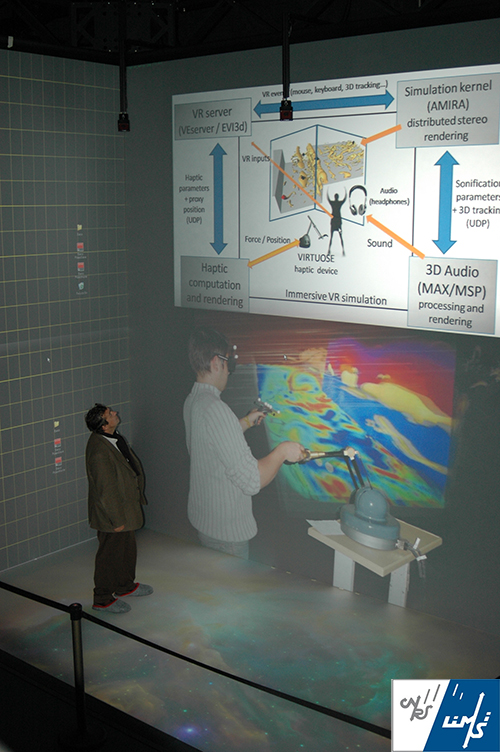
\includegraphics[width=.35\linewidth]{./figures/ch2/eve_cave_system}}
    \caption{{\it Photo de EVE, système CAVE présent au LIMSI/CNRS.}}
  \label{Fig:eve_cave_system}
  \hspace{0.3cm}
\end{figure}

\myparagraph{Dispositifs mobiles} \label{dispo_mobil}

Les visiocasques (appelés également casques immersifs ou casques de RV ou encore casques HMD for \textit{Head-Mounted Display} en anglais) sont des dispositifs se portant à la manière de casques standards et composés de deux écrans situés en face des yeux de l'utilisateur. Grâce à un système de lentilles, l'utilisateur est capable de distinguer les images affichées sur chacun des écrans de façon nette. L'affichage peut être soit monoculaire et donc perçu en 2d, soit binoculaire et donc perçu en 3d. Dans ce dernier mode, le contenu affiché sur les écrans est découpé de telle sorte que chaque œil perçoit une image différence correspondant au point de vue qui devrait être le sien dans la réalité comme illustrée dans la Figure \ref{Fig:pymol_stereo}. Le contenu affiché évolue suivant l'orientation de la tête de l'utilisateur. Cela est rendu possible par la présence d'un gyromètre calculant l'orientation relative de la tête par rapport à un point d'origine calibré au début de l'expérience. L'utilisateur possède donc une vue sur un contenu virtuel à 360 degrés qu'il peut regarder de la même façon que s'il se trouvait sur une chaise statique, mais tournant à 360 degrés. Bien que les premiers visiocasques binoculaires commercialisés datent de 1995, le domaine des casques immersifs a connu depuis quelques années un intérêt significatif de la part du monde de la recherche et du jeu vidéo. Cet intérêt peut s'expliquer par la résolution atteinte par les écrans de petite taille (type smartphone) et la précision des capteurs d'orientation utilisés pour adapter l'image à l'orientation de l'utilisateur. Du point de vue du coût, ces dispositifs sont très peu onéreux comparés aux systèmes fixes. Cependant, l'un de leurs inconvénients est le fait qu'ils dissocient l'utilisateur du monde extérieur, favorisant une utilisation solitaire.

\begin{figure}
  \centering
  {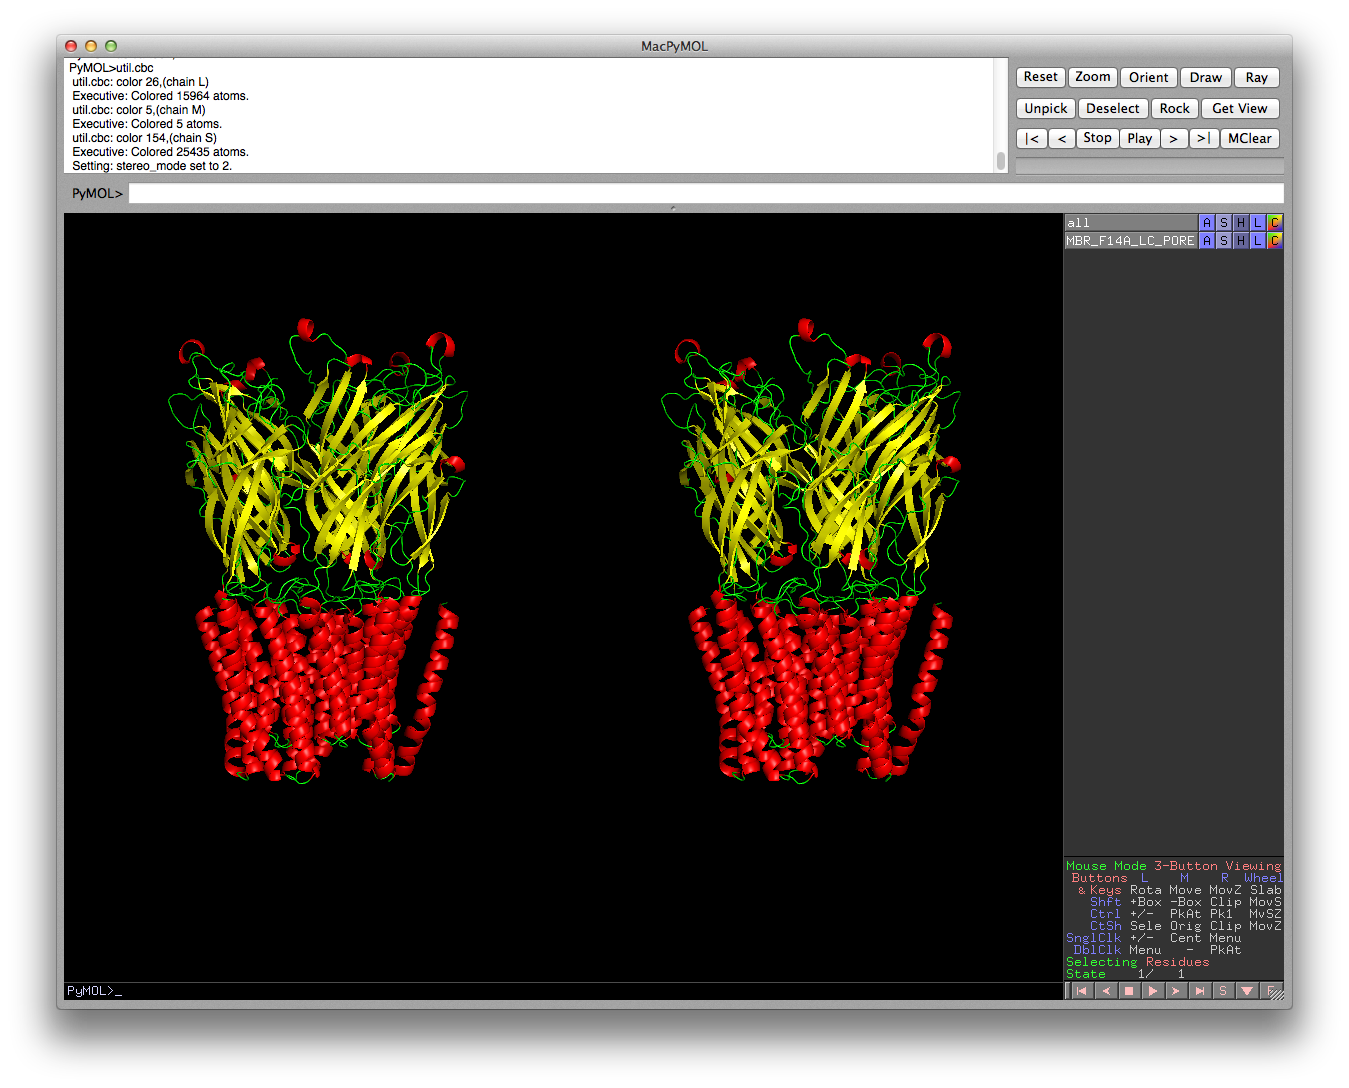
\includegraphics[width=.75\linewidth]{./figures/ch2/pymol_stereo}}
    \caption{{\it Capture d'écran de PyMol exécuté en mode stéréoscopique "cross-eyes": l'image de la protéine de droite correspond à l'oeil gauche et inversement.}}
  \label{Fig:pymol_stereo}
  \hspace{0.3cm}
\end{figure}

\subsubsection{Interfaces motrices} \label{interface_motor}

Afin de se mouvoir et d'évoluer dans le monde virtuel, l'utilisateur doit pouvoir être positionné par la plateforme de rendu. La navigation dans un environnement virtuel est une problématique cruciale en RV, d'autant plus lorsqu'elle s'effectue au sein d'un environnement virtuel abstrait et en l'absence des repères spatiaux habituellement rencontrés dans le monde réel.
Parmi les dispositifs permettant de récupérer les positions de la tête ou du corps de l'utilisateur, le \textit{tracking} optique est l'un des plus usités. Il fonctionne au moyen de caméras infrarouges et de marqueurs réfléchissants (voir Figure \ref{Fig:ir-tracking}). Des motifs de marqueurs vont servir de cibles pour les caméras infrarouges qui vont opérer une triangulation afin d'en extraire leur position. Chaque motif différent peut être associé à un objet particulier, une partie du corps ou un dispositif d'interaction. Le suivi de la tête est particulièrement utile dans les environnements immersifs puisqu'il permet de connaître la position et l’orientation de la tête et donc du regard au sein du monde virtuel. Grâce à cela, les ordinateurs responsables du rendu graphique peuvent adapter les images affichées sur les écrans pour qu'elle corresponde au point de vue de l'utilisateur dans le monde virtuel.
Il est également commun d'utiliser le système de \textit{tracking} afin de capturer les gestes de la main afin de mettre en place des interactions précises avec l'environnement. L'interaction par capture peut également se faire au travers de dispositifs d'interaction de nature variée suivant l'activité exécutée en RV. Parmi ces outils spécifiques, la souris 3d également appelée \textit{flystick} ou la manette de jeu sont couramment utilisées dans les environnements immersifs.
Enfin, il est possible de capturer l'ensemble du corps d'une personne afin de mettre en mouvement sa représentation virtuelle, appelée avatar. L'ensemble des marqueurs infrarouges va être réparti sur une combinaison afin d'obtenir la position de l'ensemble des parties mobiles du corps. Cette technique est beaucoup utilisée dans le monde du cinéma par exemple afin d'animer les avatars présents dans les films d'animation. Elle est également utilisée dans la recherche lorsque la perception de soi ou d'un collaborateur est importante pour la tâche à effectuer, par exemple au cours d'études ergonomiques.

\begin{figure}
  \centering
  {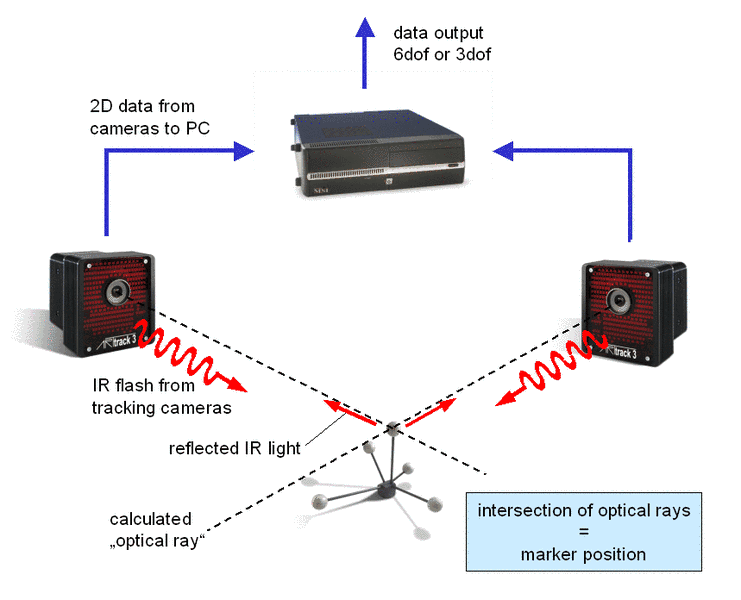
\includegraphics[width=.65\linewidth]{./figures/ch2/IR-tracking}}
    \caption{{\it Schéma simplifié d'un système de tracking optique basé sur des signaux infrarouges lancés par des caméras et se reflétant sur des marqueurs spécifiques. La configuration spatiale des marqueurs est reconnue par le PC et la position associée est calculée à partir des intersections de rayons infrarouges reflétés.}}
  \label{Fig:ir-tracking}
  \hspace{0.3cm}
\end{figure}

\subsubsection{Interfaces sensori-motrices} \label{interface_sensor-motor}

Lorsque la communication entre l'utilisateur et l'environnement est bilatérale, nous parlons d'interfaces sensori-motrices. Ces interfaces regroupent les dispositifs permettant à la fois d'interagir avec l'environnement, mais également de recevoir un stimulus sensoriel en réponse. La plus commune des interfaces sensori-motrices est l'interface haptique qui va permettre à l'utilisateur de ressentir l'effet de son interaction. Le système sensoriel haptique consiste en un ensemble de stimuli rendus à l'utilisateur et lui permettant de reconnaître un objet de façon active. Les bras à retour d'efforts permettent par exemple de manipuler des objets en 3d tout en ressentant leur poids ou d'éventuelles collisions avec d'autres objets. Le domaine médical et plus généralement des opérations télé-robotisées profitent de ces dispositifs afin de garantir un ressenti tactile complémentaire à l'information visuelle parfois limitée et/ou non suffisante. Plus généralement, les systèmes à retour d'effort impliquent une plus grande précision des gestes et des manipulations de l'utilisateur, ils sont relativement courants en conception ou simulation de pilotages, car se rapprochent au plus près des conditions réelles et usuelles.
Dans les sciences, il sont de parfaits guides pour les manipulations de systèmes biologiques interagissant sous des contraintes particulières et nécessitant d'être mis en relation de façon précise.

\subsubsection{Interactions naturelles et directes} \label{interface_nature}

Afin d'augmenter la sensation d'immersion de l'utilisateur et améliorer son expérience, il existe des interfaces dites naturelles ou directes qui vont chercher à s'inspirer des techniques d'interaction du monde réel. Le premier apport de ces interfaces est qu'elle s'adresse davantage à l'intuition de l'utilisateur que les interfaces évoquées précédemment.
Les interactions directes, regroupant les interactions mettant en jeu des mouvements de l'utilisateur ou des commandes vocales pour interagir avec son environnement virtuel, font opposition aux interactions indirectes comme peuvent l'être le clavier, la souris ou les dispositifs d'interaction immersifs comme la souris 3d ou les manettes évoquées précédemment. Ces méthodes induisent une présence moins importante des menus, favorisant ainsi davantage l'immersion. Il est bon de noter que ces interactions ont souvent une courbe d'apprentissage plus longue que les interactions indirectes. De plus, elle demande souvent une précision plus importante et est donc soumise à des variations d'efficacité parfois plus importantes. Elles sont cependant moins contraignantes pour l'utilisateur puisqu'elles ne se basent pas sur une charge matérielle autre que des supports de marqueurs pour la capture de gestes et un micro, déporté ou non, pour la reconnaissance vocale. Une fois acquises, elle permettent en plus le couplage avec d'autres moyens d'interactions et offrent donc une palette d'interactions beaucoup plus large.

La combinaison des différentes méthodes d'interaction que nous avons vue est un domaine de recherche à part entière \cite{martin_hardware_2014,martin_reconfigurable_2011}. On parle de \textbf{multimodalité} lorsqu'on propose aux utilisateurs des interactions au travers de leurs différents canaux sensori-moteurs. Cette combinaison va permettre de gérer des actions complexes et complémentaires réduisant ainsi le besoin de simplification des tâches entre les versions non-immersive et immersive d'un programme.

\section{Apports et usages de la réalité virtuelle en biologie structurale}

La RV possède plusieurs facettes répondant naturellement aux problèmes posés par l'analyse scientifique. Rappelons la problématique actuelle de la visualisation de données scientifiques. Les données générées excèdent de loin les capacités d'interprétation disponibles. De plus, la complexité et la quantité des données sont telles que leur rendu 2D ou 3d sur des écrans d'ordinateur ne sont plus suffisants pour rapporter l'ensemble des informations que les données contiennent. L'accès à certaines informations est donc entravé et enfoui sous la quantité de données à analyser par l'utilisateur.

\subsection{Perception humaine 3d}

Dans le cadre de la visualisation scientifique, on peut considérer que la capacité d'affichage stéréoscopique doublée à une surface d'affichage à 360 degrés est la facette la plus importante de la RV. Plusieurs études ont par exemple démontré que la perception de la profondeur lors de la représentation de structures moléculaires apportait une aide non négligeable pour leur compréhension structurelle \cite{van_dam_immersive_2000,stone_immersive_2010,odonoghue_visualization_2010}. Les complexes moléculaires et les protéines sont par nature structurés en 3d et c'est cette structuration qui est au cœur des études en biologie structurale. La stéréoscopie est donc une alternative naturelle pour l'observation de structures protéiques puisqu'elle utilise la compréhension innée de la 3d du cerveau humain pour analyser des phénomènes et objets de nature 3d. 
Mais l'étude de la structure seule ne peut suffire lors de l'étude d'un complexe moléculaire, nous avons souligné auparavant la présence de nombreuses données accompagnant la génération de modèles 3d lors d'une simulation moléculaire. Ces données, sous forme de valeurs brutes, doivent être également analysées. La dimension de profondeur propre à la stéréoscopie prend une nouvelle fois tout son sens ici. Ce n'est plus la nature 3d même des données observées qui va rendre cette profondeur importante, puisque nous nous intéressons maintenant à des valeurs numériques brutes, mais la possibilité d'utiliser une 3e dimension pour représenter des modèles, des tendances ou bien des anomalies au sein des données affichées.
Au-delà de la stéréoscopie, la surface, ou davantage le volume quand on parle de 3d, disponible dans les dispositifs de RV pour afficher des informations est beaucoup plus important que ce qu'on peut retrouver au sein de dispositifs 2d standards. Combiné avec un suivi de l'orientation et de la position de la tête de l'utilisateur, il devient aisé de créer un monde composé de 360 degrés d'informations accessibles simplement et rapidement au moyen d'un simple coup d'oeil.

\subsection{Interfaces sensori-motrices comme vecteurs d'informations}

La notion d'interaction n'intervient pas que dans un sens unique et même si la méthode permettant d'interagir avec un objet est primordiale, le retour sensoriel provoqué par l'interaction est, en RV, un sujet d'étude à part entière. Nous avons vu que ces retours sensoriels participent à l'immersion ressentie par l'utilisateur dans un monde virtuel, mais ils peuvent également servir de repères ou de vecteurs d'informations utilisés pour compléter les informations visuelles. Même s'il est possible de mettre en place certaines sollicitations autres que visuelles lors d'un travail sur un poste de travail standard, il est très rare de trouver des retours sonores ou haptiques lors d'une session de travail. Au-delà des limites matérielles qui peuvent exister, un retour haptique impliquant par exemple la nécessité de posséder un dispositif muni d'un système de retour d'effort, les limites sont souvent logicielles, peu de programmes implémentent des retours sensoriels autres que visuels dans le design de leurs outils d'analyses de données. Il est au contraire très commun de prendre en compte ces retours sensoriels lors du développement de solutions logicielles dédiées à la RV. La RV est par essence définie par l'implication de l'utilisateur. Il a donc dû développer très tôt des moyens pour retranscrire un maximum de sensations aux utilisateurs lors de leurs expériences virtuelles. En visualisation de données abstraites et/ou scientifiques, l'utilisation de méthodes de retours sensoriels a pu ensuite être détournée de leur but premier, l'immersion, pour communiquer des informations supplémentaires à l'utilisateur pendant ses phases d'interactions. La possibilité par exemple de déclencher un événement sonore lors de la sélection de données critiques ou extrêmes dans un set de données est l'un des exemples de l'utilisation d'un retour auditif pour transmettre une information \cite{ferey_multisensory_2009}. De la même façon, le domaine de la conception assistée par ordinateur (CAO), très présent en RV, utilise des dispositifs de retour de force afin de juger de la résistance de matériaux ou de limites de torsion/translation des objets \cite{sun2010haptic}. La chirurgie est également demandeuse de solutions précises de retours haptiques au sein de ses récentes applications de RV dédiées à l’entraînement des chirurgiens à des opérations spécifiques ou développées pour le contrôle de robots pour des opérations sur des patients réels \cite{kusumoto_application_2006}. Étendre ces moyens de fournir des informations par d'autres canaux que les canaux visuels pour la visualisation de données scientifiques en RV est donc une solution réaliste et concrète, simplifiée par les méthodes de RV déjà existantes.


\subsection{Outils et applications}

La biologie structurale n'a su que tardivement se placer par rapport à la RV. Ce n'est que très récemment que certains programmes dédiés à l'exploration moléculaire ont commencé à être utilisés au sein de dispositifs de RV \cite{odonoghue_visualization_2010}. YASARA \cite{krieger2014yasara} ou VMD \cite{stone_immersive_2010} sont deux exemples de programmes de visualisation moléculaires disponibles pour un rendu stéréoscopique et adapté aux environnements immersifs. Ils permettent l'interfaçage de leur solution de visualisation avec de nombreuses librairies utilisées en RV dans les systèmes immersifs de type CAVE ou mur d'écran. Nous pouvons citer VRPN \cite{taylor2001vrpn}, FreeVR \cite{pape2004commodity} ou VR Juggler par exemple, 3 suites de librairies. 
D'autres initiatives ponctuelles ont aussi vu le portage d'autres logiciels dans des environnements immersifs, mais ces développements spécifiques ont rarement dépassé l'extension du rendu graphique depuis le 2d jusqu'en 3d\footnote{\url{http://www.rug.nl/science-and-society/centre-for-information-technology/research/hpcv/vr\_visualisation/mol\_visualisation?lang=en}} ou la mise en place de librairies comme base de développement d'applications RV pour la visualisation moléculaire \cite{salvadori_moka:_2014}.  Afin d'améliorer l'apprentissage de certains concepts biologiques, il est parfois utile d'en améliorer la perception, en particulier quand ces concepts sont par aspects abstraits. Un projet éducatif a cherché à évaluer l'impact pour les étudiants de visualiser des objets moléculaires en RV dans le cadre de cours de biologie structurale \cite{tan_use_2013}. Selon leurs conclusions, les dispositifs immersifs ont permis un meilleur apprentissage des notions abordées ainsi qu'une compréhension globale de la biologie structurale plus complète.
La liste des applications mêlant explicitement la biologie structurale et la RV est relativement courte. Le travail d'ingénierie est par aspects déjà fait, mais il semble manquer une réflexion ergonomique autour de l'intégration des outils de biologie structurale au sein de dispositifs immersifs.


\section{Limites et perspectives en RV pour la biologie structurale} % (fold)
\label{sec:perspectives}

Nous avons souligné dans la section \ref{RV_science} les caractéristiques de la RV et ce qu'elle pouvait apporter à l'expérience de travail. A savoir qu'au-delà d'un simple rendu stéréoscopique, les enjeux d'une implémentation réussie en RV passent par la mise en place d'interactions adaptées et pertinentes pour la tâche de l'expert et au contenu qu'il manipule.

Parmi les problématiques soulevées par la RV pour les données abstraites et scientifiques, nous avons déjà évoqué le cantonnement de la discipline à des tâches d'exploration et de visualisation de structures 3d. La réalisation de tâches nécessitant une interaction avec les données mises en jeu, dans un premier temps exclusivement 3d, nécessite la mise en place de méthodes de navigation adaptées. Or la navigation au sein des mondes virtuels est l'un des obstacles cruciaux à franchir pour assurer une expérience optimale aux utilisateurs. En effet, la notion de monde virtuel implique la possibilité pour l'utilisateur d'évoluer au sein d'un environnement étendu de la même manière qu'il évoluerait dans la vie réelle. Or, si cette navigation virtuelle peut être inspiré de paradigme utilisé dans un cadre de navigation réelle dans le cas d'environnements virtuels écologiques, là où le contenu virtuel proposé est une copie artificielle d'éléments réels, la question est tout autre lorsque la scène observée n'est plus écologique et implique des éléments abstraits. 

Le caractère abstrait des objets de la biologie structurale, décidera directement de la qualité de repères spatiaux que l'utilisateur possédera pour naviguer. La visualisation moléculaire met en scène des représentations artificielles d'atomes, non observables à l’œil humain en temps normal, et dont les couleurs et formes respectent des standards décidés par le domaine, non dictés par des observations réelles. Les repères spatiaux sont donc peu nombreux et souvent trop sommaires pour assurer une orientation acceptable de l'utilisateur. Afin de combler ce manque préjudiciable pour l'expérience utilisatrice lors de ses futures tâches en biologie structurale, nous avons développé une série de paradigmes de navigation, basées sur le contenu observé et les tâches usuelles en visualisation/exploration moléculaire.

Dans la même optique de mettre en place un environnement virtuel respectant les contraintes de la RV, il nous a paru important d'adapter les interactions habituelles qu'un expert peut avoir dans des sessions de visualisation et d'analyses. Ces interactions, trop complexes et trop cloisonnées dans des environnements de bureau, doivent être simplifiées et harmonisées afin de pouvoir faire cohabiter et communiquer les étapes complémentaires que sont la visualisation et l'analyse. On remarque que dans la boucle de la VA (voir Figure \ref{Fig:visual_analytics_process_keim}), ces deux étapes sont couplées de manière très étroites proches, aussi bien en terme de données utilisées que d'implication de l'utilisateur. Leur rapprochement et fusion au sein d'un unique module est pertinent et pourrait donc se faire à travers la mise en place d'une représentation des notions utilisées dans chacune des étapes. L'utilisation d'ontologie comme illustrée précédemment permet cela et va même plus loin, car elle pourrait simplifier l'étape de \textit{transformation} des données en imposant un carcan et un vocabulaire précis aux données d'entrée. Ce deuxième pan de notre étude nous a menés à la mise en place d'une plateforme multi-composants s'appuyant sur l'utilisation d'une base de données RDF dont la structure dépend directement d'une ontologie OWL créée pour décrire notre domaine d'application.









%Comme nous l'avons souligné auparavant, la génération de données de plus en plus complexes et de plus en plus massives produite de manière expérimentales ou théorique, pose de nombreux problèmes dans les étapes suivantes, notamment en terme de visualisation et d'analyse, et d'interprétation systématique des résultats produits. 

%Lors de l'étape de modélisation, les systèmes que l'expert doit construire en amont de l'étape de simulation sont de plus en plus complexe, nécessite la manipulation dans l'espace de nombreux acteurs.

%Il convient de mettre en place de nouvelles approches pour outiller ces usages, en couplant notamment plus étroitement les processus de production de données au processus d'interprétation d'analyse des données. 



% section probl_matique (end)